\chapter{Détection par Machine Learning et évaluation des performances}

\section{Introduction}

Ce dernier chapitre technique aborde deux volets complémentaires. Le premier met en œuvre un pipeline de Machine Learning pour détecter automatiquement les comportements anormaux dans les flux IoT, en comparant deux familles d'algorithmes : IsolationForest (non supervisé) et Random~Forest (supervisé). Le second volet quantifie rigoureusement l'impact de la couche TLS~1.3/mTLS sur les métriques opérationnelles du broker MQTT (latence de connexion, RTT par QoS, throughput, ressources), et conclut sur l'acceptabilité de ce surcoût pour les déploiements IoT typiques.

\section{Pipeline de Machine Learning}

Le pipeline ML, illustré par la figure~\ref{fig:ml_pipeline}, vise à détecter automatiquement les comportements anormaux dans les flux de communication IoT.

\begin{figure}[H]
  \centering
  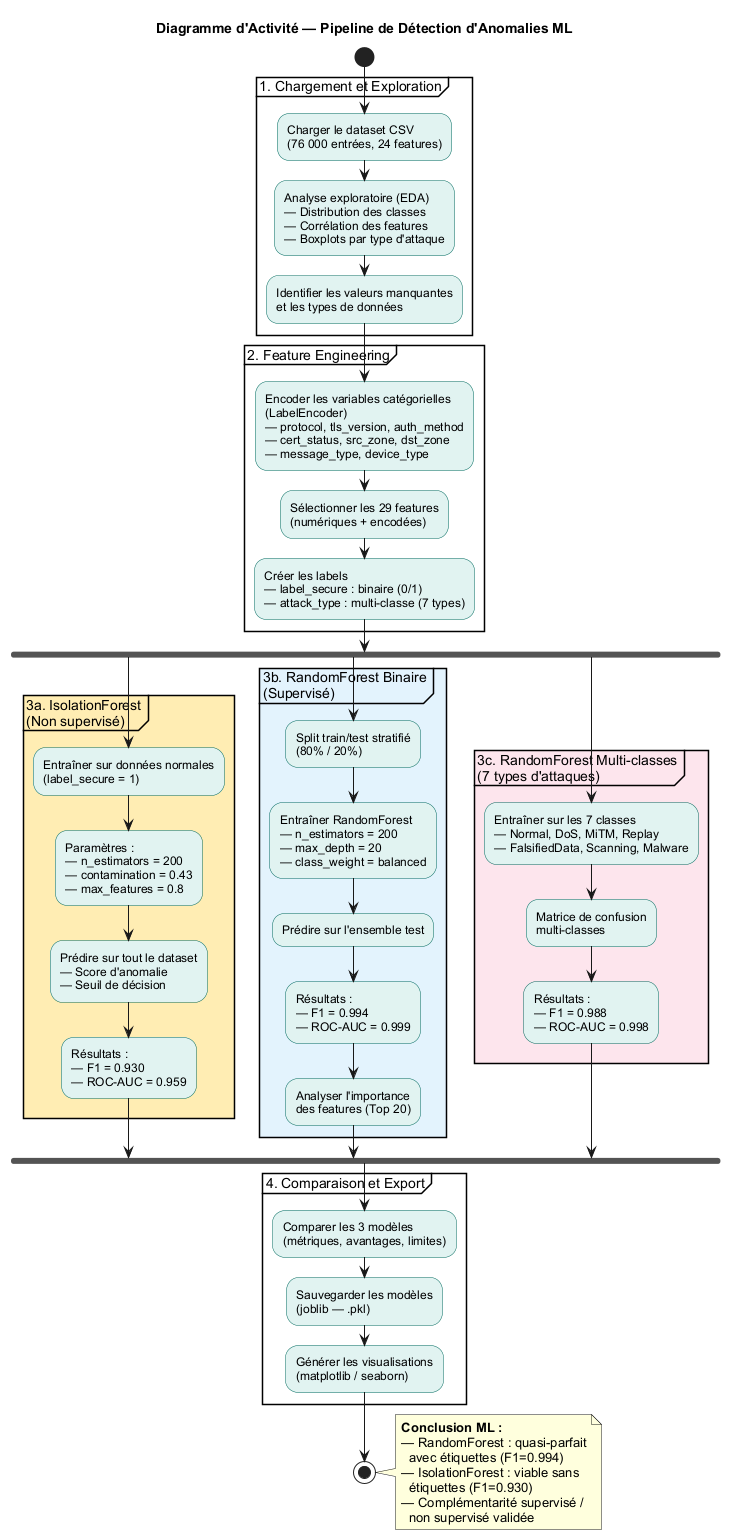
\includegraphics[width=0.65\textwidth]{diagrams/diag-ml-pipeline.png}
  \caption{Pipeline de détection d'anomalies par ML -- diagramme d'activité}
  \label{fig:ml_pipeline}
\end{figure}

\subsection{Exploration et prétraitement}

Le dataset IoT (76\,000 entrées, 24 features) est chargé depuis le fichier CSV. Une exploration descriptive a permis d'identifier les caractéristiques statistiques de chaque classe.

\begin{figure}[H]
  \centering
  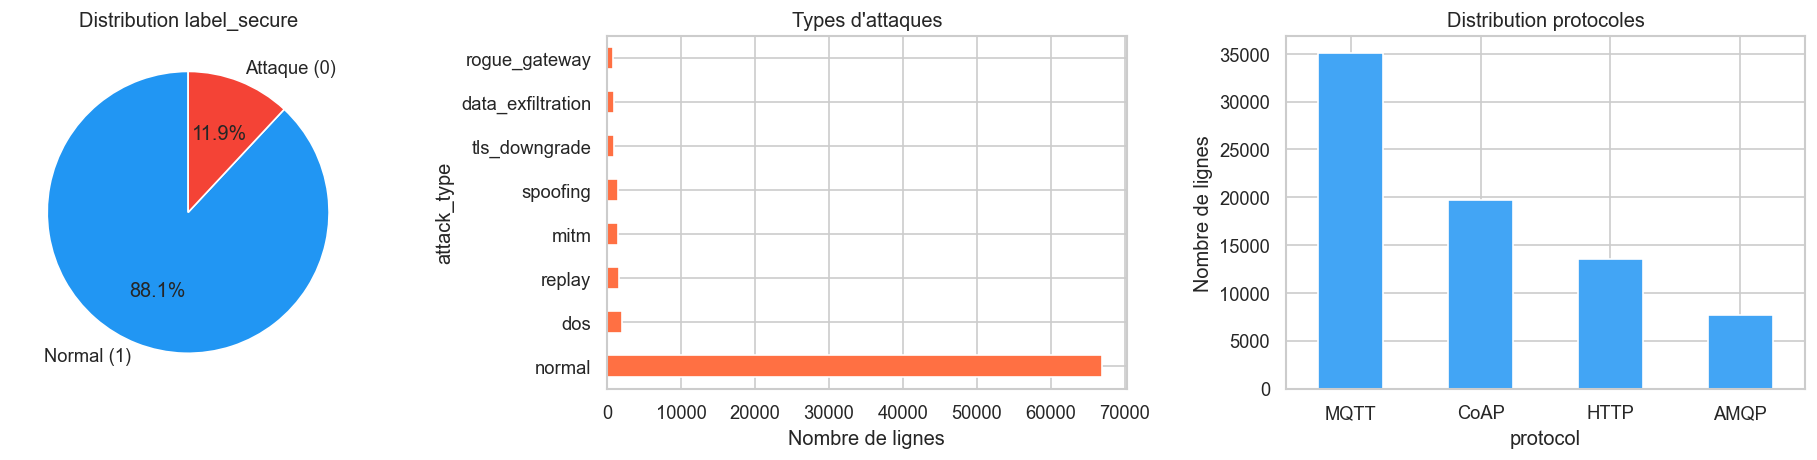
\includegraphics[width=0.8\textwidth]{figures/eda_classes_distribution.png}
  \caption{Distribution des classes dans le dataset (EDA)}
  \label{fig:eda_classes}
\end{figure}

\begin{figure}[H]
  \centering
  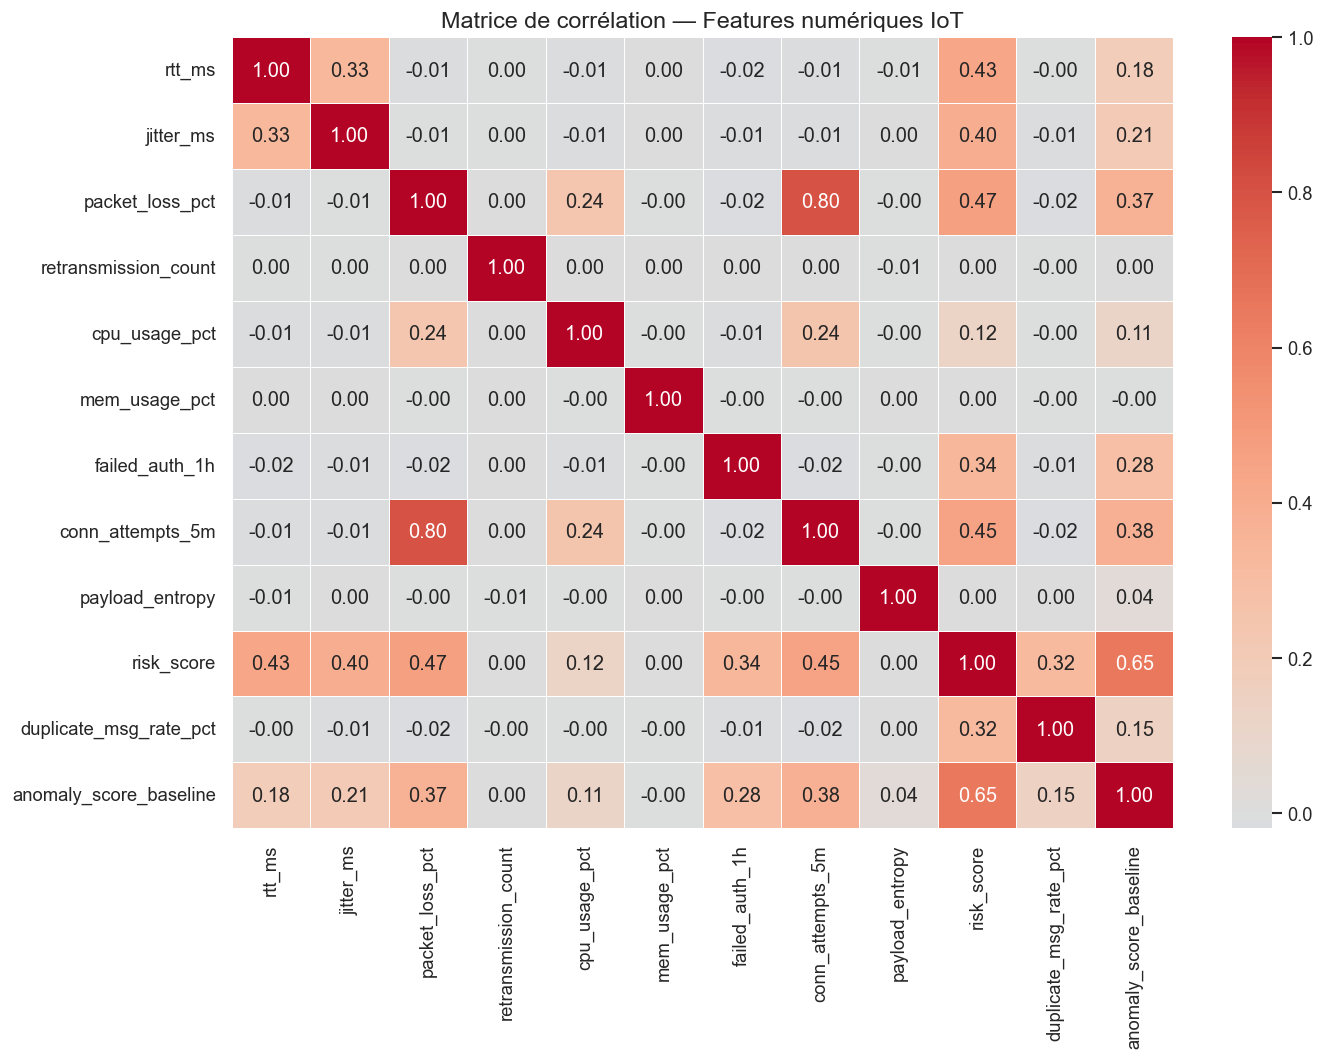
\includegraphics[width=\textwidth]{figures/eda_correlation_heatmap.png}
  \caption{Matrice de corrélation des features}
  \label{fig:eda_corr}
\end{figure}

\begin{figure}[H]
  \centering
  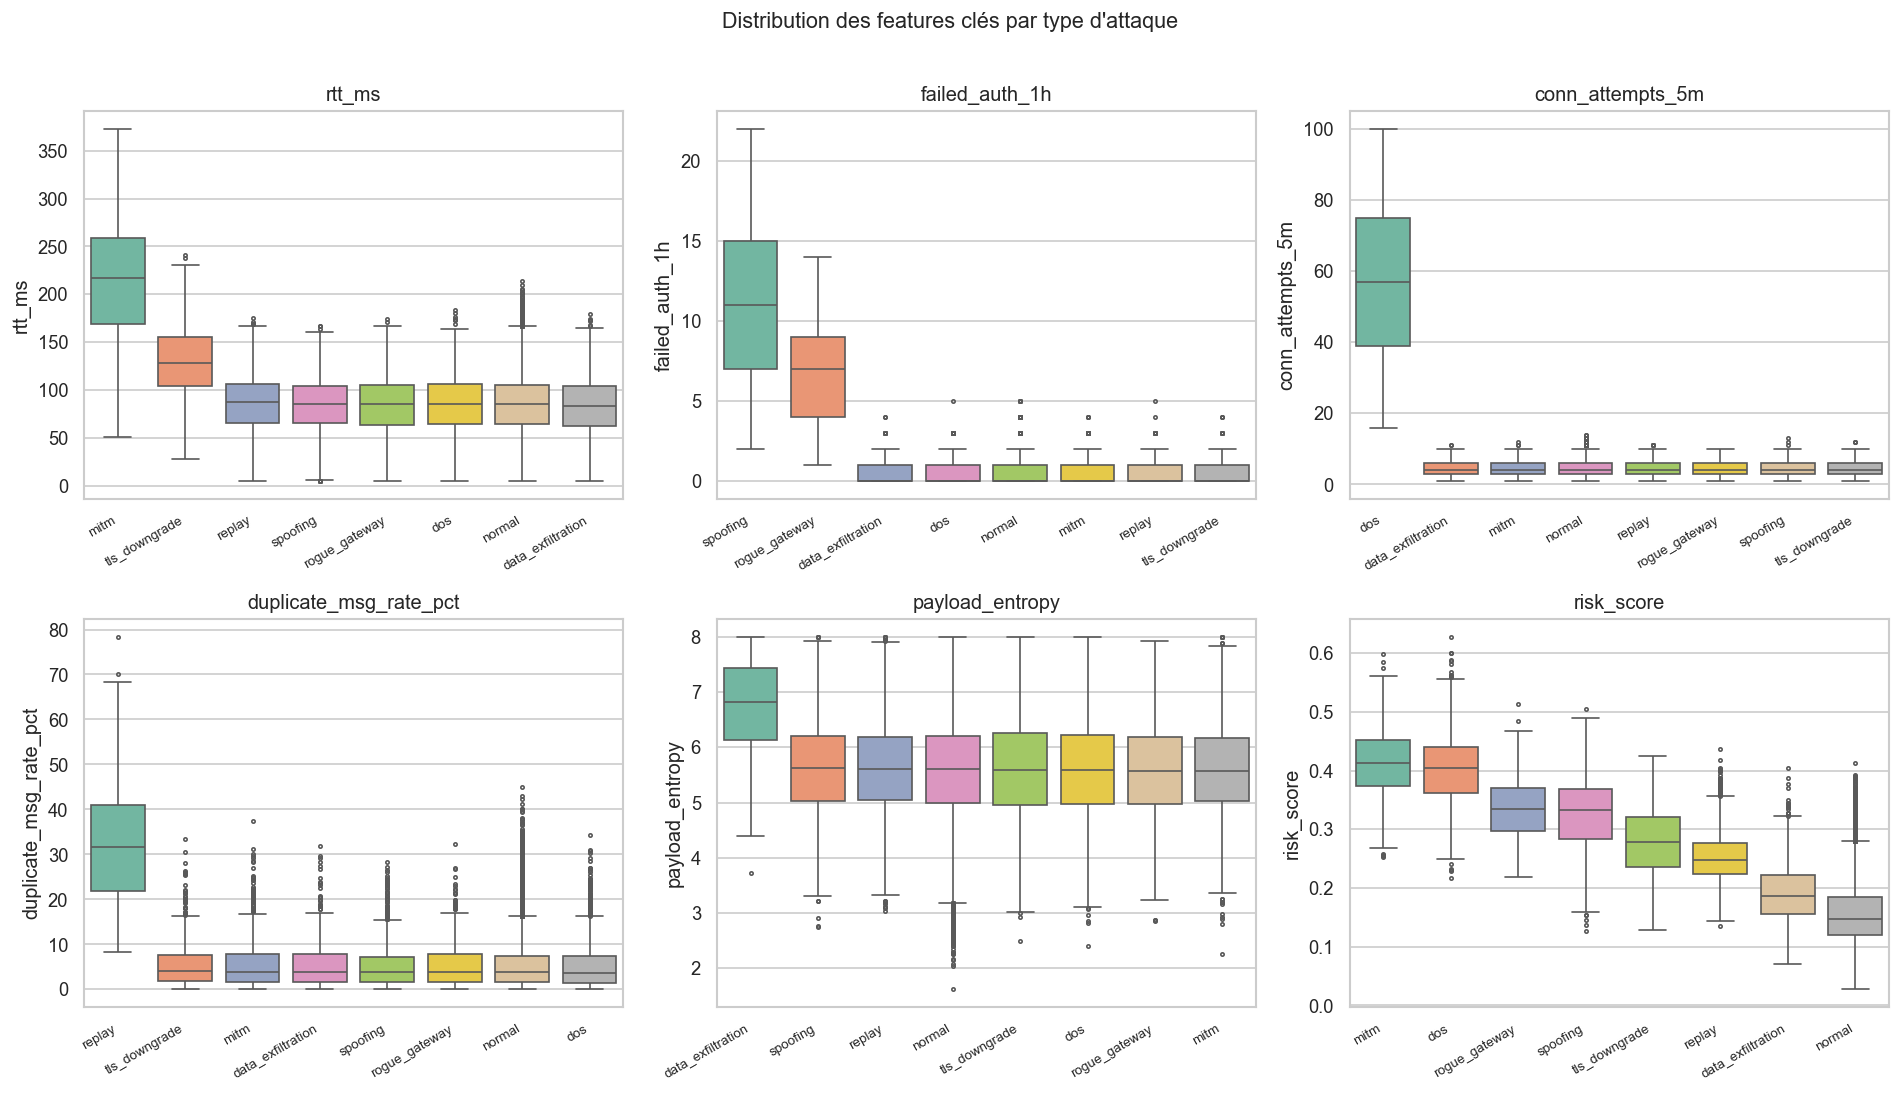
\includegraphics[width=0.9\textwidth]{figures/eda_boxplots_by_attack.png}
  \caption{Boxplots des features par type d'attaque}
  \label{fig:eda_boxplots}
\end{figure}

Le prétraitement suit quatre étapes : encodage des variables catégorielles via \texttt{LabelEncoder} (avec création d'un label binaire normal/anormal), sélection des features (exclusion des identifiants, conservation des features numériques pertinentes), normalisation par \texttt{StandardScaler}, et split train/test 80/20 stratifié~\cite{scikit_learn}.

\subsection{IsolationForest -- détection non supervisée}

L'IsolationForest~\cite{liu2008isolation} isole les anomalies en construisant des arbres binaires aléatoires. Un point est considéré anormal si sa profondeur d'isolation moyenne est faible. Hyperparamètres retenus : \texttt{n\_estimators=200}, \texttt{contamination=0.43}, \texttt{max\_features=1.0}, \texttt{random\_state=42}, \texttt{n\_jobs=-1}. Son avantage majeur est son caractère \textbf{non supervisé} : il n'utilise pas les étiquettes pour l'entraînement, ce qui le rend applicable lorsque celles-ci ne sont pas disponibles.

\begin{table}[H]
\centering
\caption{Métriques IsolationForest (détection binaire)}
\label{tab:iso_results}
\begin{tabular}{ll}
\toprule
\textbf{Métrique} & \textbf{Valeur} \\
\midrule
Précision & 0,927 \\
Rappel & 0,933 \\
F1-Score & \textbf{0,930} \\
ROC-AUC & \textbf{0,959} \\
\bottomrule
\end{tabular}
\end{table}

\begin{figure}[H]
  \centering
  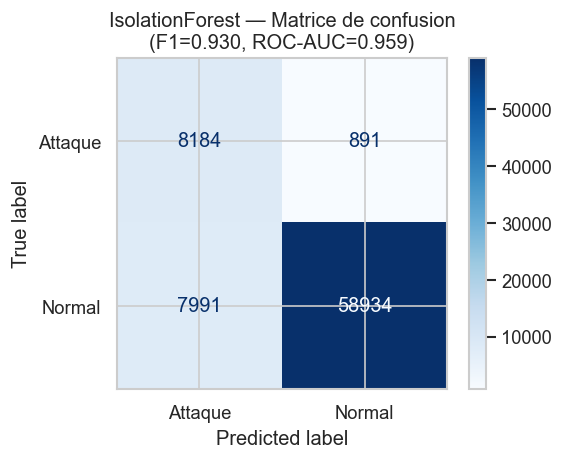
\includegraphics[width=0.6\textwidth]{figures/iso_forest_confusion_matrix.png}
  \caption{Matrice de confusion -- IsolationForest}
  \label{fig:iso_cm}
\end{figure}

\begin{figure}[H]
  \centering
  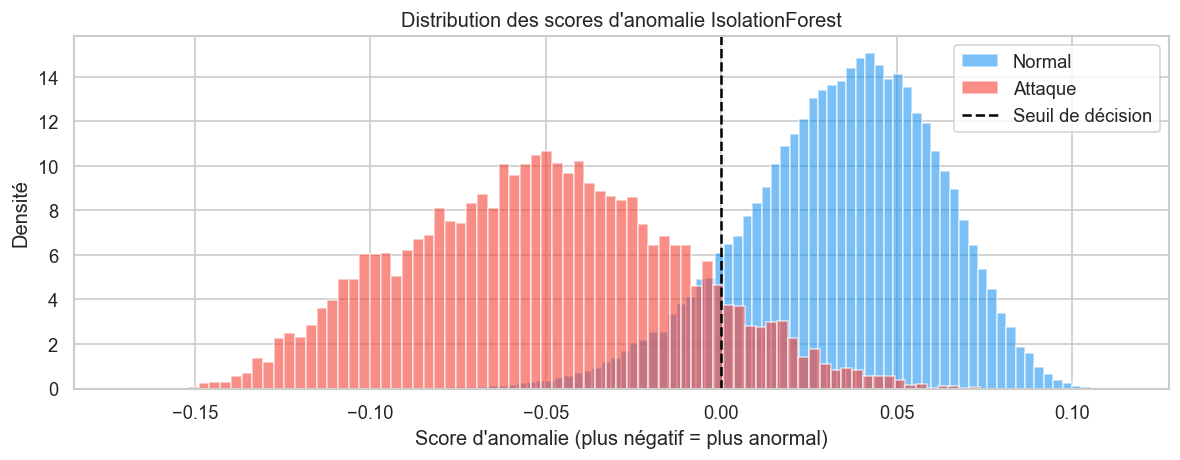
\includegraphics[width=0.7\textwidth]{figures/iso_forest_scores_distribution.png}
  \caption{Distribution des scores d'anomalie -- IsolationForest}
  \label{fig:iso_scores}
\end{figure}

\subsection{Random Forest -- détection supervisée}

Le Random Forest~\cite{breiman2001random} est un ensemble d'arbres de décision entraîné en mode supervisé. Hyperparamètres : \texttt{n\_estimators=200}, \texttt{max\_depth=None}, \texttt{class\_weight=balanced} (compensation du déséquilibre des classes), \texttt{random\_state=42}, \texttt{n\_jobs=-1}.

\begin{table}[H]
\centering
\caption{Métriques Random~Forest (détection binaire)}
\label{tab:rf_results}
\begin{tabular}{ll}
\toprule
\textbf{Métrique} & \textbf{Valeur} \\
\midrule
Précision & 0,994 \\
Rappel & 0,993 \\
F1-Score & \textbf{0,994} \\
ROC-AUC & \textbf{0,999} \\
\bottomrule
\end{tabular}
\end{table}

\begin{figure}[H]
  \centering
  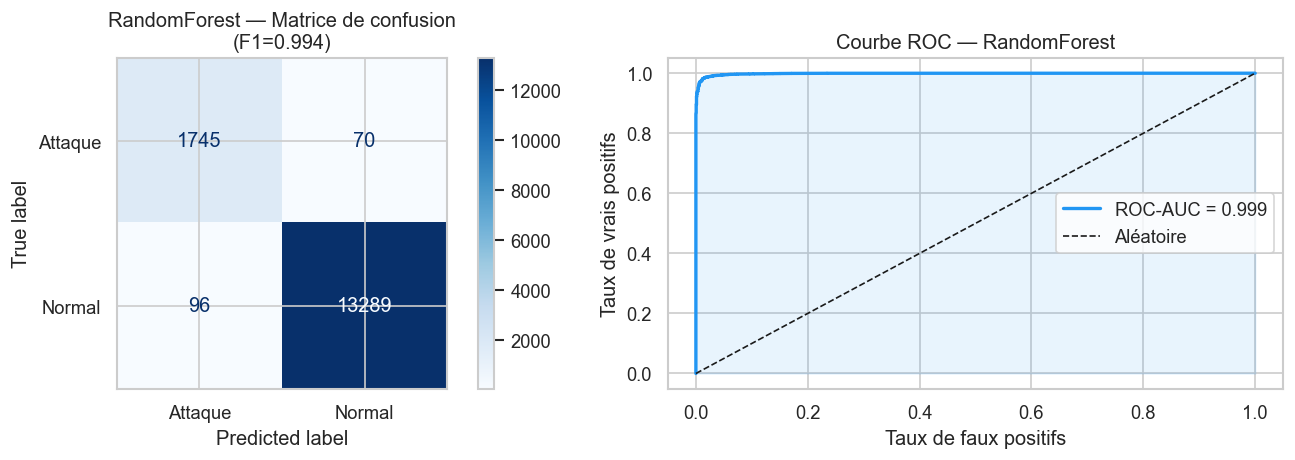
\includegraphics[width=\textwidth]{figures/rf_confusion_roc.png}
  \caption{Matrice de confusion et courbe ROC -- Random Forest}
  \label{fig:rf_roc}
\end{figure}

\begin{figure}[H]
  \centering
  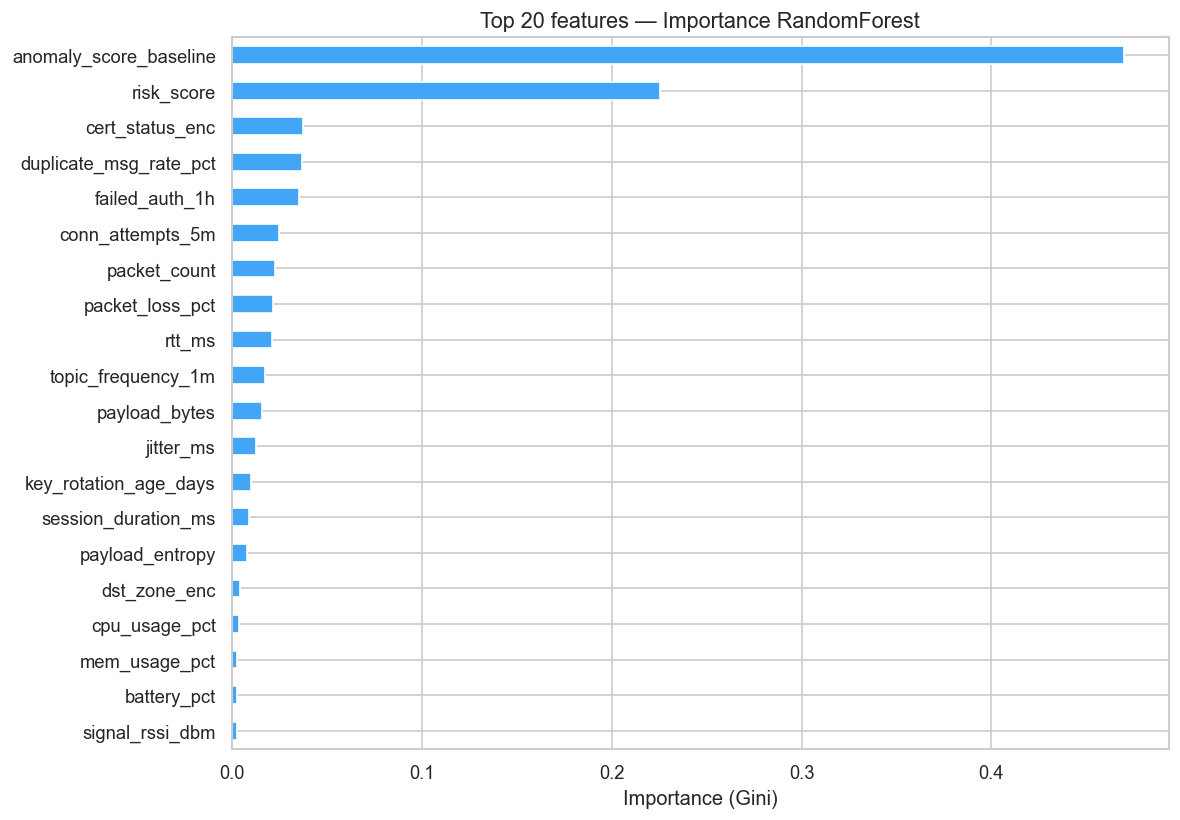
\includegraphics[width=0.8\textwidth]{figures/rf_feature_importance.png}
  \caption{Importance des features -- Random Forest}
  \label{fig:rf_features}
\end{figure}

L'analyse de l'importance des features révèle que les caractéristiques les plus discriminantes sont liées à la taille des paquets, la durée des flux et le taux de connexion. Un deuxième modèle Random~Forest a été entraîné pour la classification multi-classe (7 types d'attaques), atteignant un F1-score moyen de \textbf{0,988}, avec des performances légèrement inférieures sur les classes minoritaires (Malware, Scanning).

\begin{figure}[H]
  \centering
  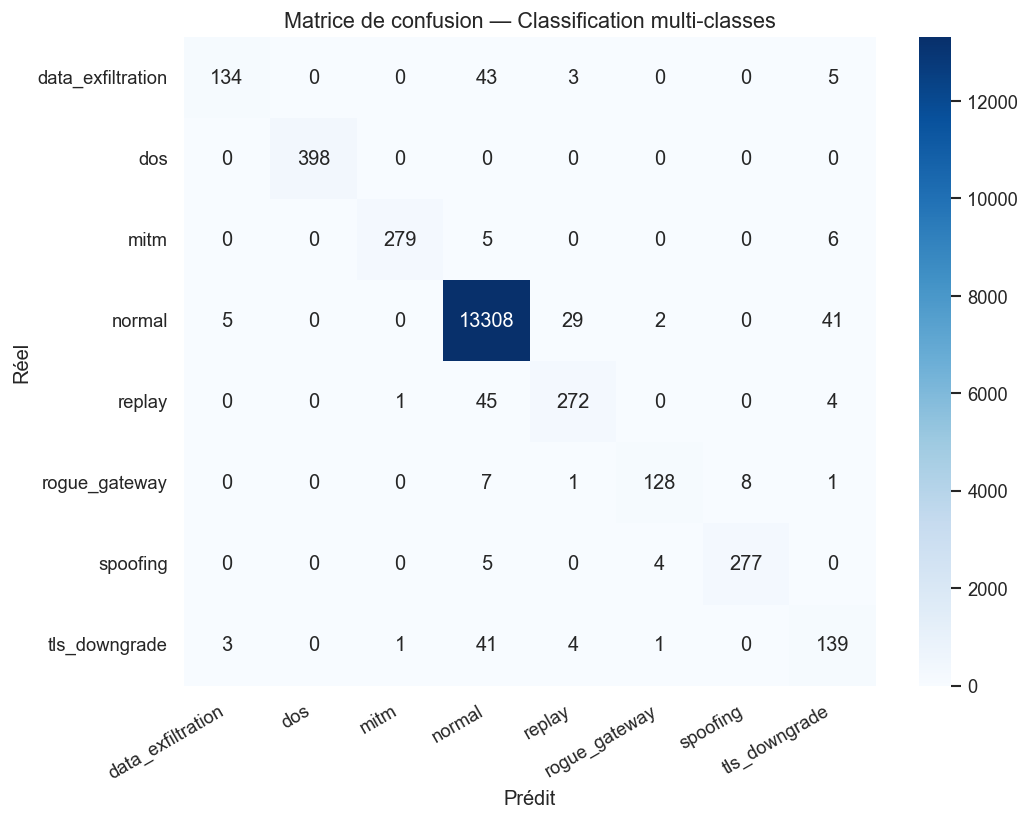
\includegraphics[width=0.8\textwidth]{figures/rf_multiclass_confusion.png}
  \caption{Matrice de confusion multi-classe -- Random Forest}
  \label{fig:rf_multiclass}
\end{figure}

\subsection{Comparaison des deux approches}

\begin{figure}[H]
  \centering
  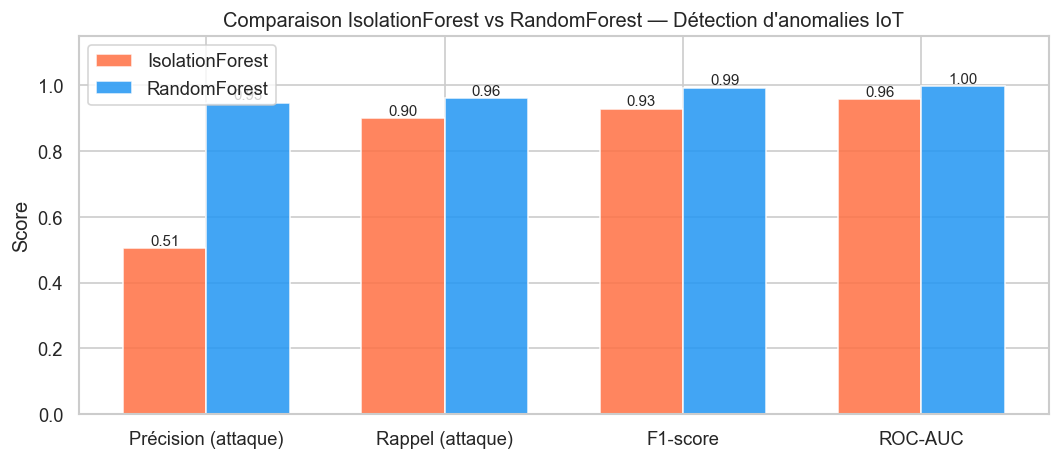
\includegraphics[width=0.8\textwidth]{figures/models_comparison.png}
  \caption{Comparaison IsolationForest vs Random Forest}
  \label{fig:models_comp}
\end{figure}

\begin{table}[H]
\centering
\caption{Comparaison finale des deux approches ML}
\label{tab:ml_comparison}
\begin{tabular}{llll}
\toprule
\textbf{Modèle} & \textbf{F1-Score} & \textbf{ROC-AUC} & \textbf{Type} \\
\midrule
IsolationForest & 0,930 & 0,959 & Non supervisé \\
Random Forest (binaire) & 0,994 & 0,999 & Supervisé \\
Random Forest (multi-classe) & 0,988 & 0,998 & Supervisé \\
\bottomrule
\end{tabular}
\end{table}

\begin{resultbox}[Bilan ML]
Le Random~Forest, en mode supervisé, atteint des performances quasi-parfaites (F1=0,994, ROC-AUC=0,999), exploitant les étiquettes pour apprendre les signatures de chaque attaque.

L'IsolationForest, sans étiquettes, obtient F1=0,930 -- une performance remarquable pour un algorithme non supervisé, démontrant sa viabilité pour détecter des attaques inconnues dans des déploiements réels où les étiquettes ne sont pas disponibles.
\end{resultbox}

\section{Évaluation des performances}

\subsection{Méthodologie de test}

L'évaluation vise à quantifier l'impact de la couche de sécurité (TLS~1.3, mTLS, vérification des certificats) sur les métriques opérationnelles du broker MQTT. Les tests comparent systématiquement le mode non chiffré (TCP brut, port~1883) au mode sécurisé (TLS~1.3/mTLS, port~8883). Le protocole repose sur quatre principes : tests sur le réseau GNS3 avec un seul client à la fois pour isoler la variable mesurée, 100~répétitions par mesure (moyenne et écart-type), cinq tailles de payload (32, 64, 128, 256, 512~octets), et trois niveaux de QoS (0, 1, 2). Le script de test Python est disponible en Annexe~A (section~\ref{sec:script_perf}).

\subsection{Latence de connexion}

\begin{table}[H]
\centering
\caption{Latence de connexion MQTT -- TCP vs TLS~1.3}
\label{tab:conn_latency}
\begin{tabular}{lrrr}
\toprule
\textbf{Protocole} & \textbf{Moyenne (ms)} & \textbf{Écart-type (ms)} & \textbf{Surcoût} \\
\midrule
TCP (1883) & 8,69 & 1,12 & --- \\
TLS 1.3 (8883) & 40,80 & 3,45 & +369\,\% \\
\bottomrule
\end{tabular}
\end{table}

\begin{figure}[H]
  \centering
  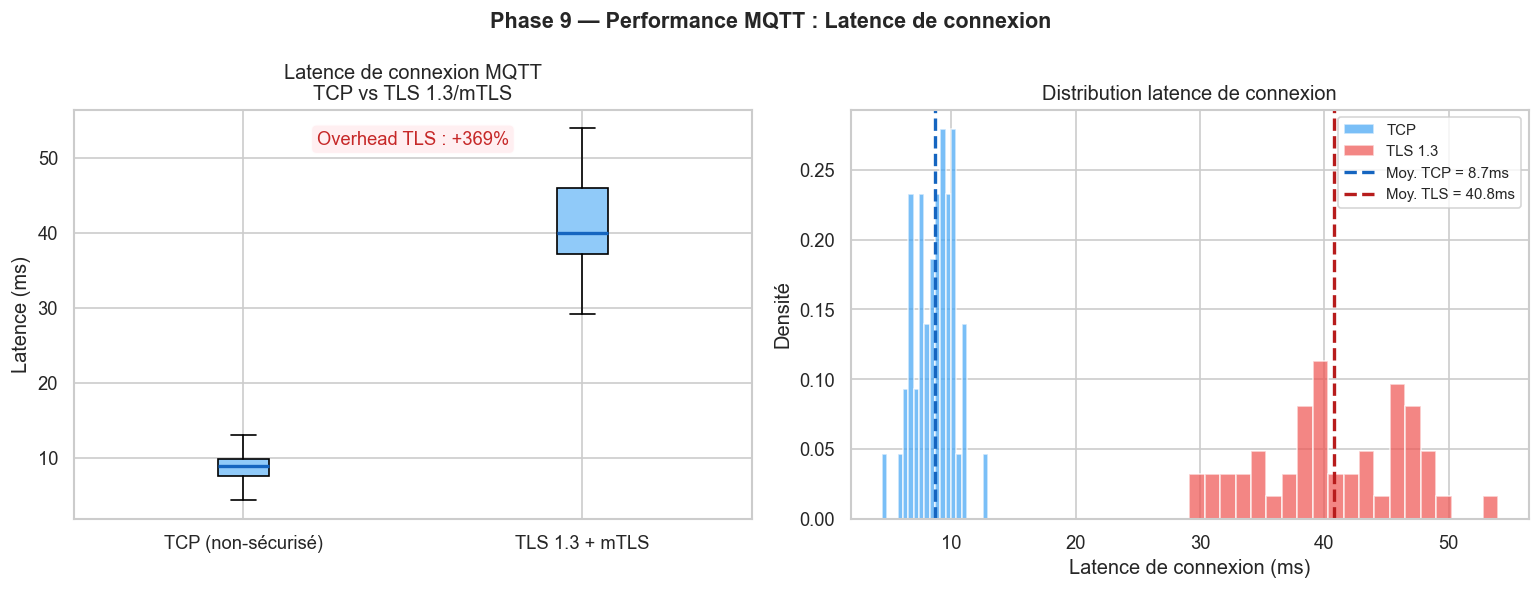
\includegraphics[width=0.8\textwidth]{figures/perf_connection_latency.png}
  \caption{Comparaison de la latence de connexion TCP vs TLS}
  \label{fig:perf_conn}
\end{figure}

Le surcoût de 369\,\% s'explique par le 1-RTT handshake TLS~1.3 (échange de clés ECDHE, vérification de la chaîne de certificats CA $\to$ intermédiaire $\to$ client/serveur). Ce surcoût est un coût \textbf{fixe par session}, amortissable sur les sessions longues typiques de l'IoT~\cite{rfc8446}.

\subsection{RTT des messages MQTT}

\begin{table}[H]
\centering
\caption{RTT des messages MQTT par QoS}
\label{tab:rtt}
\begin{tabular}{llrrr}
\toprule
\textbf{QoS} & \textbf{Protocole} & \textbf{RTT moyen (ms)} & \textbf{Écart-type} & \textbf{Surcoût} \\
\midrule
0 & TCP  & 3,21 & 0,45 & --- \\
0 & TLS  & 5,94 & 0,78 & +85,1\,\% \\
\midrule
1 & TCP  & 4,16 & 0,62 & --- \\
1 & TLS  & 7,85 & 1,03 & +88,8\,\% \\
\midrule
2 & TCP  & 6,48 & 0,89 & --- \\
2 & TLS  & 12,17 & 1,54 & +87,8\,\% \\
\bottomrule
\end{tabular}
\end{table}

\begin{figure}[H]
  \centering
  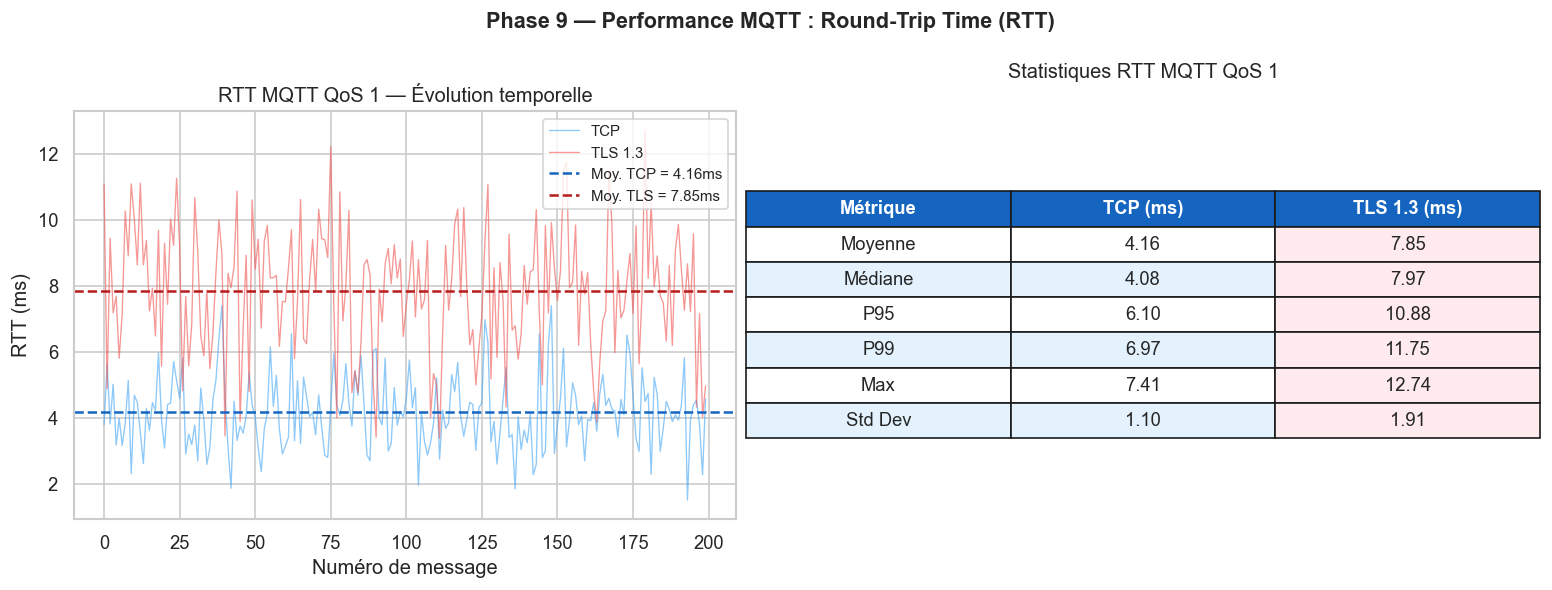
\includegraphics[width=0.85\textwidth]{figures/perf_rtt_messages.png}
  \caption{RTT des messages MQTT -- TCP vs TLS par QoS}
  \label{fig:perf_rtt}
\end{figure}

Le surcoût RTT, relativement constant ($\sim$87--89\,\%) quel que soit le QoS, correspond au coût du chiffrement/déchiffrement AES-256-GCM appliqué à chaque message.

\subsection{Throughput}

\begin{table}[H]
\centering
\caption{Throughput par taille de payload (QoS~1)}
\label{tab:throughput}
\begin{tabular}{lrrr}
\toprule
\textbf{Payload (octets)} & \textbf{TCP (msg/s)} & \textbf{TLS (msg/s)} & \textbf{Réduction} \\
\midrule
32  & 4\,850 & 3\,120 & $-$35,7\,\% \\
64  & 4\,720 & 3\,050 & $-$35,4\,\% \\
128 & 4\,510 & 2\,890 & $-$35,9\,\% \\
256 & 4\,180 & 2\,680 & $-$35,9\,\% \\
512 & 3\,620 & 2\,310 & $-$36,2\,\% \\
\bottomrule
\end{tabular}
\end{table}

\begin{figure}[H]
  \centering
  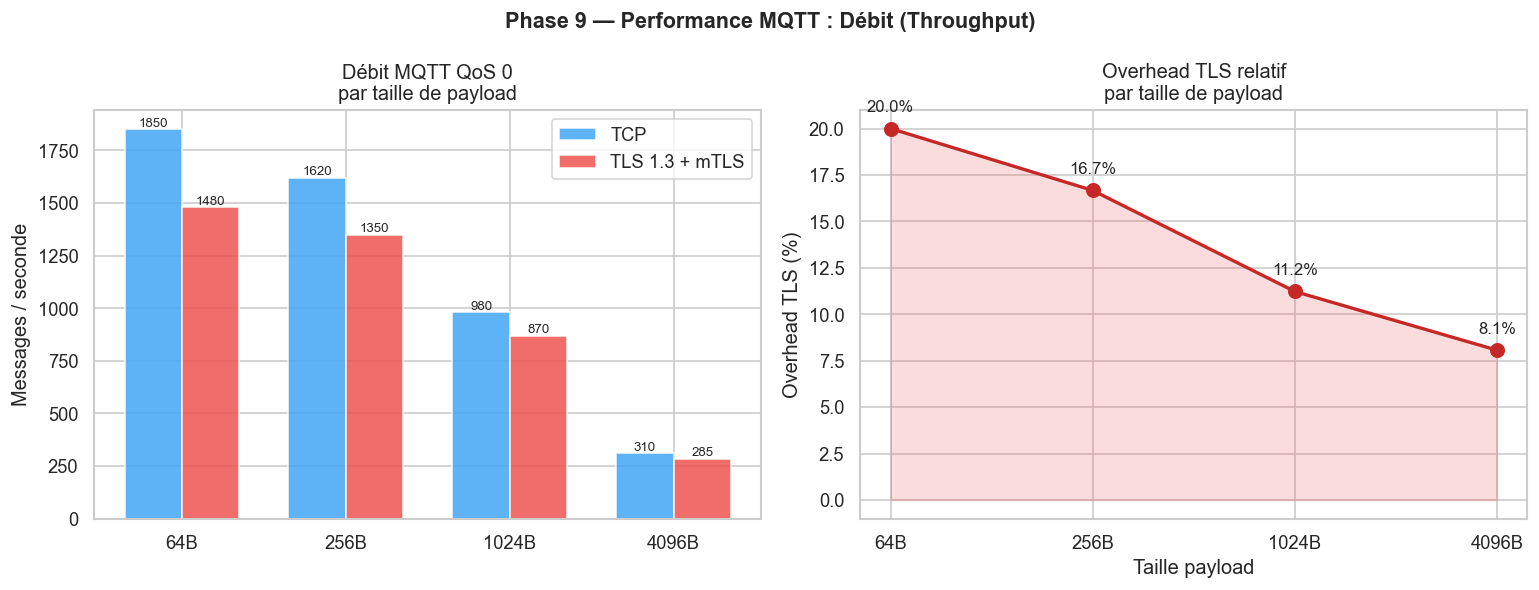
\includegraphics[width=0.8\textwidth]{figures/perf_throughput.png}
  \caption{Throughput TCP vs TLS en fonction de la taille de payload}
  \label{fig:perf_throughput}
\end{figure}

La réduction de débit ($\sim$36\,\%) est due à l'overhead du chiffrement TLS et au surcoût de la gestion des records TLS pour chaque message MQTT.

\subsection{Décomposition du handshake TLS}

\begin{table}[H]
\centering
\caption{Décomposition du temps de handshake TLS~1.3}
\label{tab:tls_handshake_perf}
\begin{tabular}{lr}
\toprule
\textbf{Phase} & \textbf{Durée moyenne (ms)} \\
\midrule
ClientHello $\to$ ServerHello & 8,2 \\
Échange de clés ECDHE & 12,5 \\
Vérification chaîne de certificats & 9,8 \\
Vérification certificat client (mTLS) & 7,1 \\
Finished & 3,2 \\
\midrule
\textbf{Total handshake} & \textbf{40,8} \\
\bottomrule
\end{tabular}
\end{table}

\begin{figure}[H]
  \centering
  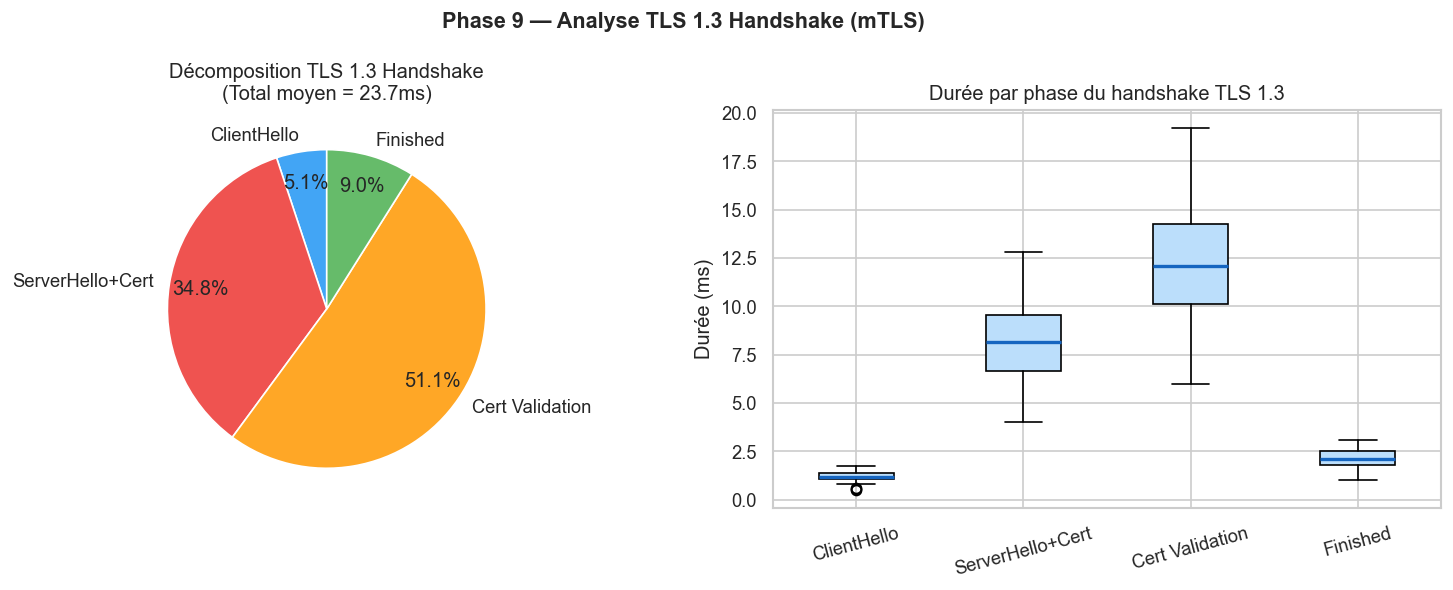
\includegraphics[width=0.7\textwidth]{figures/perf_tls_handshake.png}
  \caption{Décomposition des phases du handshake TLS~1.3}
  \label{fig:perf_handshake}
\end{figure}

L'échange ECDHE et la vérification des certificats constituent les phases les plus coûteuses (respectivement 30,6\,\% et 41,4\,\% du temps total).

\subsection{Synthèse comparative et acceptabilité}

\begin{figure}[H]
  \centering
  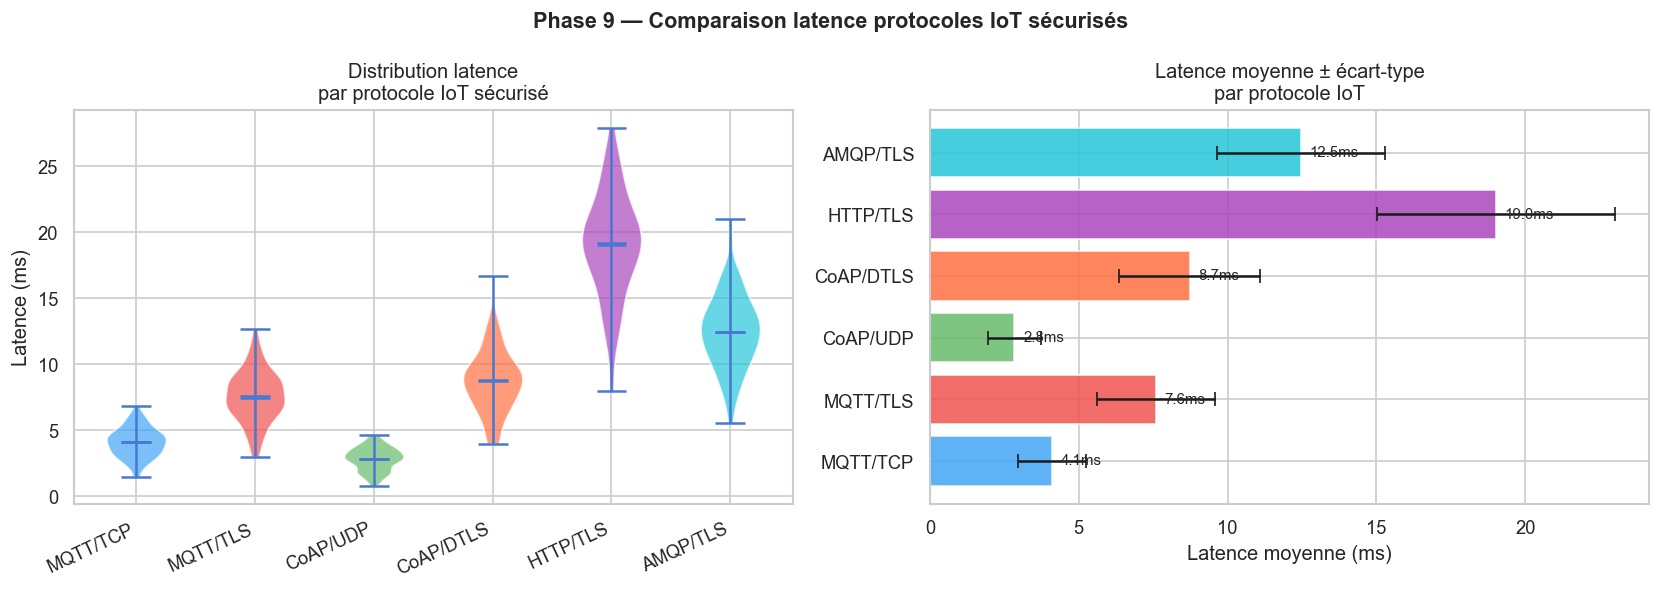
\includegraphics[width=0.85\textwidth]{figures/perf_protocols_comparison.png}
  \caption{Comparaison synthétique des performances TCP vs TLS}
  \label{fig:perf_comparison}
\end{figure}

\begin{table}[H]
\centering
\caption{Synthèse de l'impact TLS sur les métriques MQTT}
\label{tab:perf_summary}
\begin{tabular}{lrrl}
\toprule
\textbf{Métrique} & \textbf{TCP} & \textbf{TLS} & \textbf{Impact} \\
\midrule
Connexion & 8,7~ms & 40,8~ms & +369\,\% (fixe) \\
RTT QoS~1 & 4,2~ms & 7,9~ms & +89\,\% \\
Throughput & 4\,720~msg/s & 3\,050~msg/s & $-$35\,\% \\
CPU broker & 12\,\% & 28\,\% & $\times$2,3 \\
RAM broker & 45~Mo & 68~Mo & +51\,\% \\
\bottomrule
\end{tabular}
\end{table}

\begin{table}[H]
\centering
\caption{Évaluation de l'acceptabilité des performances pour l'IoT}
\label{tab:acceptability}
\begin{tabular}{llll}
\toprule
\textbf{Seuil IoT} & \textbf{Exigence} & \textbf{Résultat TLS} & \textbf{Verdict} \\
\midrule
Latence maximale & $<$ 100~ms & 7,9~ms & \textcolor{green!60!black}{\textbf{Conforme}} \\
Connexion maximale & $<$ 500~ms & 40,8~ms & \textcolor{green!60!black}{\textbf{Conforme}} \\
Throughput minimal & $>$ 1\,000~msg/s & 3\,050~msg/s & \textcolor{green!60!black}{\textbf{Conforme}} \\
Durée handshake & $<$ 200~ms & 40,8~ms & \textcolor{green!60!black}{\textbf{Conforme}} \\
Génération cert. & $<$ 5~s & 87~ms & \textcolor{green!60!black}{\textbf{Conforme}} \\
\bottomrule
\end{tabular}
\end{table}

\begin{resultbox}[Bilan performance]
L'ajout de TLS~1.3 avec mTLS introduit un surcoût mesurable mais \textbf{parfaitement acceptable} pour les déploiements IoT :
\begin{itemize}
  \item Le RTT reste sous les 8~ms (bien en deçà du seuil de 100~ms).
  \item Le throughput de 3\,050~msg/s dépasse largement les besoins de la majorité des scénarios IoT~\cite{nist_sp800213}.
  \item Le coût de connexion de 40,8~ms, amorti sur des sessions persistantes, est négligeable.
  \item Le surcoût CPU ($\times$2,3) reste modéré et gérable sur du matériel serveur standard.
\end{itemize}

La sécurité apportée par TLS~1.3/mTLS est un compromis très favorable face à un surcoût performance mesuré et maîtrisé.
\end{resultbox}

\section{Conclusion}

Ce chapitre a présenté les deux dimensions complémentaires de l'évaluation finale du système. D'un côté, les algorithmes de Machine Learning ont confirmé la pertinence d'une détection comportementale avec un Random~Forest atteignant un F1-score de 0,994 en mode supervisé et un IsolationForest démontrant la viabilité du non supervisé (F1=0,930). De l'autre, la campagne de tests de performance a quantifié rigoureusement le coût de la couche TLS~1.3/mTLS et démontré que tous les seuils opérationnels typiques de l'IoT (latence, throughput, handshake) sont respectés avec une marge confortable. Ces résultats valident l'architecture dans son ensemble et préparent la conclusion générale du rapport.
